\section{RF Two-Port Amplifiers}
\subsection{Biasing}
\todo{Figure out what goes here}
\subsection{Stability}
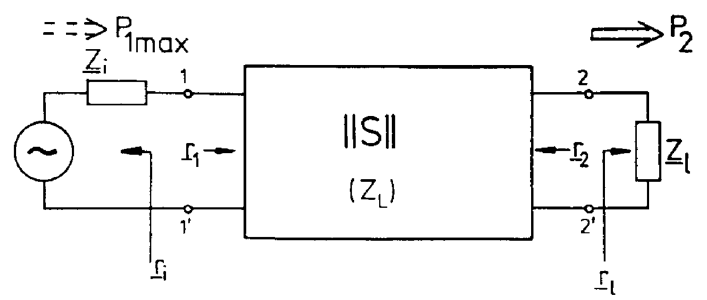
\includegraphics[width=.3\textwidth]{content/hfcomp/pictures/2-port_amplifier.png}
\begin{equation*}
    r_i = \dfrac{Z_i - Z_L}{Z_i + Z_L}, \quad r_l = \dfrac{Z_l - Z_L}{Z_l + Z_L},
\end{equation*}
\begin{equation*}
    r_1 = S_{11} + \dfrac{S_{12}S_{21}r_l}{1 - S_{22}r_l}, \quad r_2 = S_{22} + \dfrac{S_{12}S_{21}r_i}{1 - S_{11}r_i},
\end{equation*}
\begin{align*}
    g_T &= \dfrac{P_2}{P_{1,\mathrm{max}}}\\
    &=\dfrac{|S_{21}|^2 (1 - |r_i|^2) (1 - |r_l|^2)}{\left|(1 - S_{11}r_i)(1 - S_{22}r_l) - S_{12}S_{21} r_i r_l\right|^2}
\end{align*}
\begin{itemize}
    \itemsep0pt
    \item Stability Circles of Two-Port Amplifiers, with center point $\sigma$ and radius $\tau$:
        \begin{align*}
            &\text{Generator-side:}\\
            &\sigma_i = \dfrac{(S_{11} - \det(S) S_{22}^*)^*}{|S_{11}|^2 - |\det(S)|^2},\;
            \tau_i = \left|\dfrac{S_{12} S_{21}}{|S_{11}|^2 - |\det(S)|^2}\right|\\
            &\text{Load-side:}\\
            &\sigma_l = \dfrac{(S_{22} - \det(S) S_{11}^*)^*}{|S_{22}|^2 - |\det(S)|^2},\;
            \tau_l = \left|\dfrac{S_{12} S_{21}}{|S_{22}|^2 - |\det(S)|^2}\right|
        \end{align*}
    \item \textbf{Unconditional Stability for:}
        \begin{equation*}
            K = \dfrac{1 - |S_{11}|^2 - |S_{22}|^2 + |\det(S)|^2}{2 |S_{12}| |S_{21}|} > 1,
        \end{equation*}
        \begin{equation*}
            \text{and } |\det(S)| < 1.
        \end{equation*}.
\end{itemize}

\subsection{Unilateral Design of Two-Port-Amplifiers}
\begin{itemize}
    \item \textbf{Assume:} $S_{12} = 0$!
    \item Unilateral transducer power gain:
        \begin{equation*}
            g_{Tu,\mathrm{max},\mathrm{max}} = \frac{|S_{21}|^2}{(1 - |S_{11}|^2)(1 - |S_{22}|^2)}
        \end{equation*}
\end{itemize}
